% This work by Jeremy A. Hansen is licensed under a Creative Commons 
% Attribution-NonCommercial-ShareAlike 3.0 Unported License, 
% as described at http://creativecommons.org/licenses/by-nc-sa/3.0/legalcode

The C++ Standard Library, which builds upon the older Standard Template Library (STL), provides a set of tools beyond those that are provided by the ``base'' C++ language. 
While a comprehensive discussion of the features of the Standard Library is far beyond the scope of this text, there are several libraries that offer extremely important features with which you should become comfortable. 

\noindent Note: rather than assuming that 

\noindent\begin{minipage}{\linewidth}\begin{lstlisting}
using namespace std;
\end{lstlisting}\end{minipage}

\noindent is at the top of every code example, each data type, function, or variable derived from the Standard Library will be shown with the prefix \Code{std::}. 
This highlights which parts of the examples below come from the Standard Library, and which are part of the language.

\LevelD{\Code{\#include <utility>} \\ \Code{\#include <tuple>} (C++11)}

The \Code{pair} class, found in \Code{<utility>}, links two values which may be of different types. 
The \Code{tuple} class, introduced in C++11, links any number of values which may be of different types. 
For example, to link a student's identification number (an integer) and their grade point average (a \Code{float}), we can write:

\noindent\begin{minipage}{\linewidth}\begin{lstlisting}
std::pair<int,float> grades = { 112233, 3.81 };
\end{lstlisting}\end{minipage}

\noindent We can assign different values to the \Code{pair} later with the \Code{make\_pair} function: \nopagebreak[4]

\noindent\begin{minipage}{\linewidth}\begin{lstlisting}
grades = std::make_pair(123450, 2.79);
\end{lstlisting}\end{minipage}

The \Code{first} and \Code{second} members are used to extract the individual components of the \Code{pair}:

\noindent\begin{minipage}{\linewidth}\begin{lstlisting}
std::cout << "ID: " << grades.first << " (GPA " 
  << grades.second << ")" << std::endl;
// This prints:
// ID: 123450 (GPA 2.79)
\end{lstlisting}\end{minipage}

If we wanted a more complicated set of values linked together, such as a student's name, identification number, grade point average, and major, we could construct the following:

\noindent\begin{minipage}{\linewidth}\begin{lstlisting}
tuple<std::string, int, float, std::string> ethan = 
  { "Ethan Allen", 802802, 3.15, "Engineering"};
\end{lstlisting}\end{minipage}

Unfortunately, the \Code{tuple} class does not have \Code{first} or \Code{second} members. 
The first and second elements can be retrieved in a slightly more complicated way than with \Code{pair} objects:

\noindent\begin{minipage}{\linewidth}\begin{lstlisting}
std::cout << std::get<0>(ethan) << "'s major is " 
  << std::get<3>(ethan) << std::endl;
// This prints:
// Ethan Allen's major is Engineering
\end{lstlisting}\end{minipage}

In the code below, the \Code{get} function returns a reference to the third element (the GPA) of the \Code{tuple ethan}, and sets that value to 3.99:

\noindent\begin{minipage}{\linewidth}\begin{lstlisting}
std::get<2>(ethan) = 3.99;
\end{lstlisting}\end{minipage}

These types may not be all that useful by themselves, but are often used in conjunction with container classes like \Code{vector} and \Code{map}, described below.

\LevelD{\#include <iterator>}

Iterators are objects that refer to elements within a container object (like \Code{std::vector}, \Code{std::map}, and \Code{std::array}) and allow for traversal through those elements. 
The list of features in iterators vary depending on the container class. 
While the specifics of the iterators vary, most iterators belong to one of the following categories, based on the operations that may be performed on them.

\LevelE{Forward iterators}

\begin{itemize}
	\item Can be incremented to move forward in the container to the next item
	\item Can be dereferenced like a pointer variable
\end{itemize}

\noindent\begin{minipage}{\linewidth}\begin{lstlisting}
std::array<int> myArray = { 5, 10, 15, 20, 25 };
std::array::iterator myIterator, arrayEnd;
arrayEnd = myArray.end();

// Demonstrating forward iteration
for (myIterator = myArray.begin(); 
     myIterator != arrayEnd; 
     ++myIterator)
  std::cout << *myIterator << " ";

std::cout << std::endl << "The end!" << std::endl;

// This prints:
// 5 10 15 20 25
// The end!
\end{lstlisting}\end{minipage}

\LevelE{Bidirectional iterators}

\begin{itemize}
	\item Everything a forward iterator can do and:
	\item Can be decremented to move backward in the container to the previous item
\end{itemize}

\noindent\begin{minipage}{\linewidth}\begin{lstlisting}
std::array<int> myArray = { 5, 10, 15, 20, 25 };
std::array::iterator myIterator, arrayBegin;
arrayBegin = myArray.begin();

// Demonstrating backward iteration
for (myIterator = myArray.end(); 
     myIterator != arrayBegin; 
     --myIterator)
  std::cout << *myIterator << " ";

std::cout << std::endl << "The beginning!" << std::endl;

// This prints:
// 25 20 15 10 5
// The beginning!
\end{lstlisting}\end{minipage}

\LevelE{Random access iterators}

\begin{itemize}
	\item Everything a bidirectional iterator can do and:
	\item Can use arithmetic operators to move forward and backward a certain number of items at once
	\item Allows comparisons between iterators to determine relative positions in the container
	\item Can use array-style access to elements in the container
\end{itemize}

\noindent\begin{minipage}{\linewidth}\begin{lstlisting}
// Create an array of 5 integers
std::array<int, 5> myArray = { 5, 10, 15, 20, 25 };
std::array<int, 5>::iterator myIterator, arrayEnd;
arrayEnd = myArray.end();
myIterator = myArray.begin();

// Demonstrating random access
std::cout << myIterator[1] << " " 
  << myIterator[3] << std::endl;

// Demonstrating iterator comparisons
if (myIterator < arrayEnd)
  std::cout << "Not at the end of the array yet!"
    << std::endl;

// Demonstrating arithmetic operations on an iterator
for (myIterator = myArray.begin();
     myIterator != arrayEnd;
     myIterator += 2)
  std::cout << *myIterator << " ";

std::cout << std::endl << "The end!" << std::endl;

// This prints:
// 10 20
// Not at the end of the array yet!
// 5 15 25
// The end!
\end{lstlisting}\end{minipage}

\LevelD{\#include <vector>}

Vectors are containers similar to arrays that are flexible in size and quite fast. 
While we can use iterators as above, we can also treat the \Code{vector} much like an array.

\noindent\begin{minipage}{\linewidth}\begin{lstlisting}
// Start with 10 elements, all with the value 98.6
std::vector<float> temperatures(10, 98.6); 

// The last element has a fever of 103.1 degrees!
temperatures[9] = 103.1; 

for (int i = 0; i < temperatures.size(); i++)
{
  std::cout << "Patient " << i << "'s temperature is " 
    << temperatures[i] << std::endl;
}
\end{lstlisting}\end{minipage}

The \Code{vector} class also provides member functions \Code{front()} and \Code{back()} which return references to the first element and the last element in the vector, respectively.
For example:

\noindent\begin{minipage}{\linewidth}\begin{lstlisting}
std::cout << "The last patient's temperature is " 
  << temperatures.back() << std::endl;
std::cout << "The first patient's temperature is " 
  << temperatures.front() << std::endl;
\end{lstlisting}\end{minipage}

Don't confuse the \Code{back()} and \Code{front()} functions with the \Code{end()} and \Code{begin()} functions. 
The \Code{back()} and \Code{front()} functions return references to the elements, while \Code{end()} and \Code{begin()} return \emph{iterators} pointing to those elements.

\LevelD{\#include <map>}

This library provides one of the Standard Library's associative container object classes. 
An associative container differs from an array in that items in an array are referenced with a number which indicates the item's position in memory:

\noindent\begin{minipage}{\linewidth}\begin{lstlisting}
int myArray[10]; // An array of ten integers
myArray[0] = -5; // Set the first integer in the array to -5
\end{lstlisting}\end{minipage}

An associative container, on the other hand, can use any data type to reference the items in the container. 
For example, you might choose to use a \Code{string} to reference a collection of \Code{int} items to store a list of students' ages according to their names.

\noindent\begin{minipage}{\linewidth}\begin{lstlisting}
std::map<std::string,int> students;
\end{lstlisting}\end{minipage}

Perhaps you want to create the object with some initial values: \nopagebreak[4]

\noindent\begin{minipage}{\linewidth}\begin{lstlisting}
std::map<std::string,int> students = 
  { {"John", 19}, 
    {"Max", 19}, 
    {"Christine", 20}, 
    {"Maria", 18} };
\end{lstlisting}\end{minipage}

This code produces a structure like in Figure \ref{fig:STL-map-diagram}. 
With these names and ages paired, we can now retrieve the ages using the names.

\begin{figure}[tb]
  \centering
  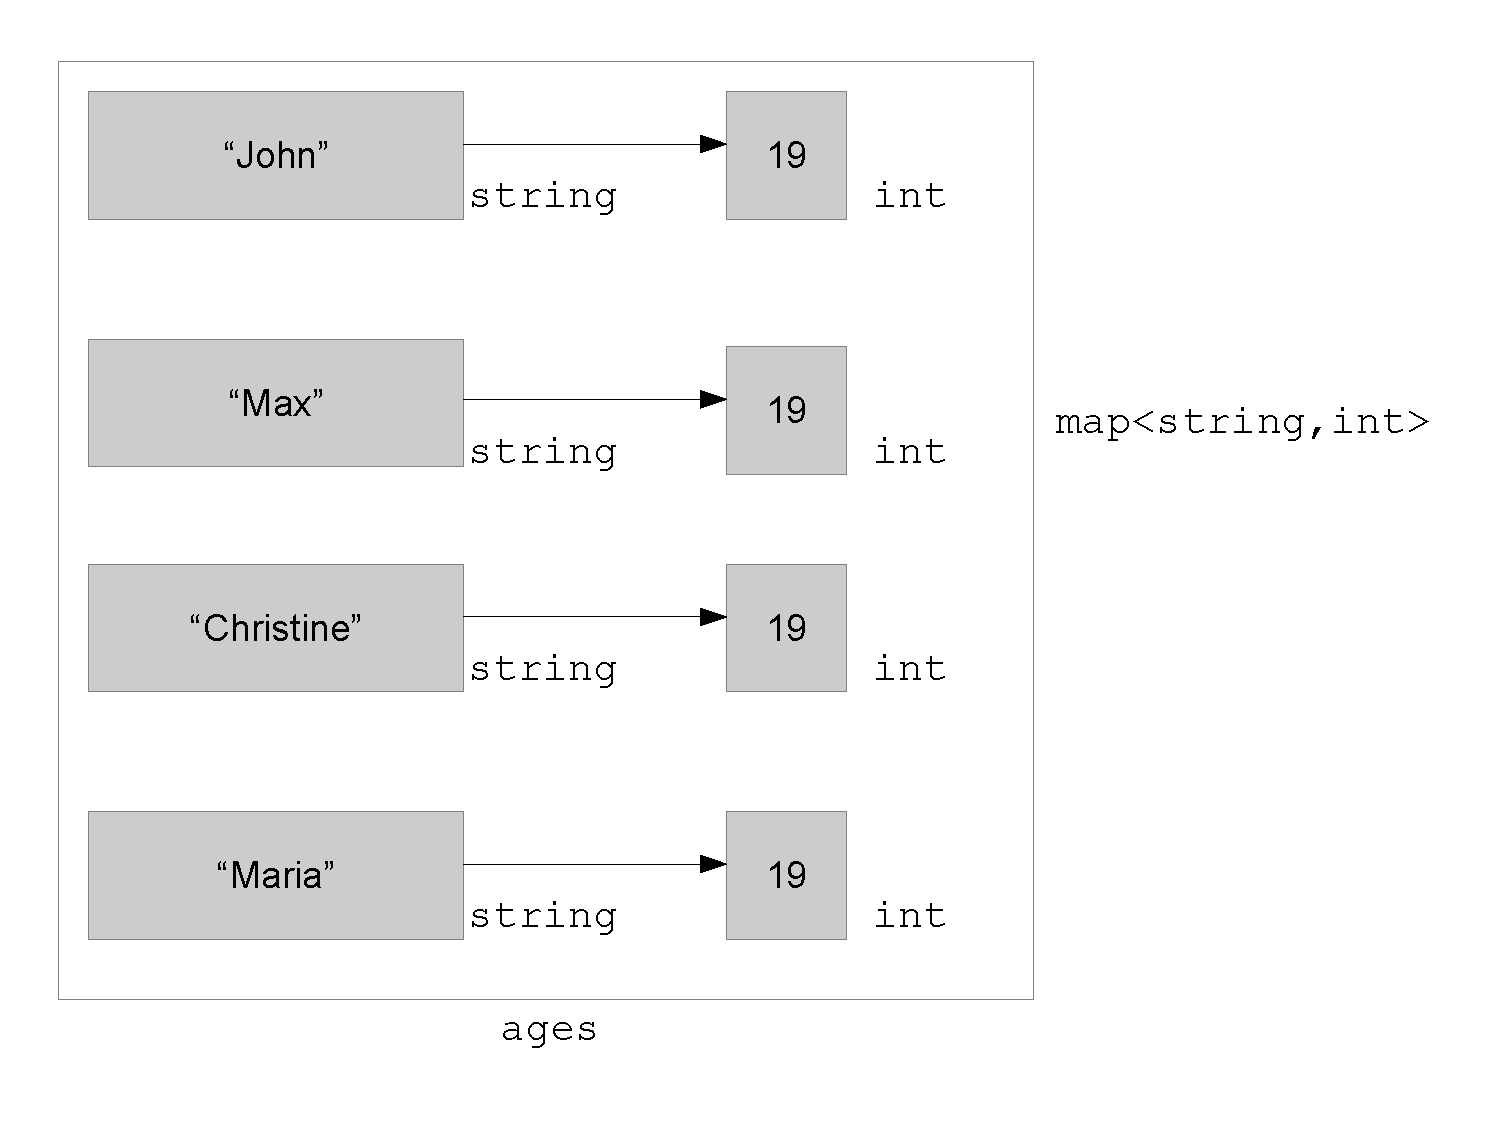
\includegraphics[width=0.8\textwidth]{diagrams/STL-map-diagram.pdf}
  \caption{Pairing \Code{string}s and \Code{int}s in a \Code{map} object} \label{fig:STL-map-diagram} 
\end{figure}

\noindent\begin{minipage}{\linewidth}\begin{lstlisting}
string name = "Christine";
std::cout << name << " is " << students[name] 
  << " years old." << std::endl;

//This code prints:
//Christine is 20 years old.
\end{lstlisting}\end{minipage}

\noindent New students may also be added in the following way:

\noindent\begin{minipage}{\linewidth}\begin{lstlisting}
students["June"] = 18;
students["Omar"] = 19;
\end{lstlisting}\end{minipage}

Objects of type \Code{map} may be iterated, and in C++11, their contents can be printed in a range-based \Code{for} loop as we briefly demonstrate here. 
Each item in the \Code{std::map<std::string, int>} is of type \Code{std::pair<std::string,int>}.

\noindent\begin{minipage}{\linewidth}\begin{lstlisting}
for (auto& item : students)
{
  std::cout << item.first << " is " << item.second << " years old." << std::endl;
}

// This code prints:
// John is 19 years old
// Max is 19 years old
// Christine is 20 years old
// Maria is 18 years old
// June is 18 years old
// Omar is 19 years old
\end{lstlisting}\end{minipage}



%\LevelD{Review Questions}

%\LevelD{Review Answers}

\LevelD{Further Reading}

\begin{itemize}
\item \url{http://en.wikipedia.org/wiki/Standard_Template_Library}
\item \url{http://www.cplusplus.com/reference/stl/}
\end{itemize}	
